%
% File poltext2016.tex
%
% Contact: jan.snajder@fer.hr or dsirinic@gmail.com
%%
%% Based on the style files for ACL-2015, which were, in turn,
%% Based on the style files for ACL-2014, which were, in turn,
%% Based on the style files for ACL-2013, which were, in turn,
%% Based on the style files for ACL-2012, which were, in turn,
%% based on the style files for ACL-2011, which were, in turn, 
%% based on the style files for ACL-2010, which were, in turn, 
%% based on the style files for ACL-IJCNLP-2009, which were, in turn,
%% based on the style files for EACL-2009 and IJCNLP-2008...

%% Based on the style files for EACL 2006 by 
%%e.agirre@ehu.es or Sergi.Balari@uab.es
%% and that of ACL 08 by Joakim Nivre and Noah Smith

\documentclass[11pt]{article}
\usepackage{poltext2016}
\usepackage{times}
\usepackage{url}
\usepackage{latexsym}
\usepackage{booktabs}
\usepackage{graphicx} % more modern
%\usepackage{epsfig} % less modern
\usepackage{subfigure}

\usepackage{natbib}
\usepackage{amsmath,amsfonts,amscd,amssymb}
\usepackage{dsfont}
\renewcommand{\vec}[1]{\mathbf{#1}}
\usepackage{hyperref}
\DeclareMathOperator*{\argmax}{argmax}
\DeclareMathOperator*{\argmin}{argmin}
\DeclareMathOperator*{\Corr}{Corr}
\newcommand{\R}{\mathds{R}}
\usepackage{multicol}
\usepackage{multirow}
\usepackage{pbox}
\usepackage{color}

% As of 2011, we use the hyperref package to produce hyperlinks in the
% resulting PDF.  If this breaks your system, please commend out the
% following usepackage line and replace \usepackage{icml2015} with
% \usepackage[nohyperref]{icml2015} above.
\usepackage{hyperref}

% Packages hyperref and algorithmic misbehave sometimes.  We can fix
% this with the following command.
\newcommand{\theHalgorithm}{\arabic{algorithm}}


\newcommand{\pola}[1]{\textcolor{blue}{#1}}
\newcommand{\felix}[1]{\textcolor{green}{#1}}

%\setlength\titlebox{5cm}

% You can expand the titlebox if you need extra space
% to show all the authors. Please do not make the titlebox
% smaller than 5cm (the original size); we will check this
% in the camera-ready version and ask you to change it back.

\title{Predicting political party affiliation from text}

\author{Felix Biessmann\\
%  {\tt felix.biessmann@gmail.com} \\ 
  \And
  Sebastian Schelter\\
  Technische Universit\"at Berlin\\
%  {\tt sebastian.schelter@tu-berlin.de}\\
\And 
Daniel Kirsch
  \And
 Pola Lehmann \\
  Wissenschaftszentrum Berlin \\
%  {\tt pola.lehmann@wzb.eu} \\
  }

\date{}

\begin{document}
\maketitle


\begin{abstract}
Every day large amounts of text are produced in public discourse. Some of this text is produced by actors whose political colour is very obvious, for example in the case of party elites. But there are also many actors raising their voices in the discourse, who cannot be clearly attributed to a political party, while their statements might actually by biased towards a specific party. Identifying such biases is crucial for political research as well as media consumers, especially when analysing the influence of the media on political discourse and vice versa. In this study we investigate to what extent political party affiliation can be predicted from textual content. Results indicate that automatic classification of political affiliation is possible with above chance accuracy also across text domains. We propose methods to better interpret these results and find that features not related to political policies, such as speech sentiment, can be discriminative and thus exploited by text analysis models. 
%We present an example of a web application that combines topic modelling with automatic political affiliation analyses of news articles based on the proposed model.
\end{abstract}

\section{Introduction}
\label{sec:intro}
%
Analysis and classifications of political text is and has been a very important tool to generate political science data (Benoit et al. 2015). Traditionally such classifications are done by experts, who read and label the text of interest.\footnote{See for example the Manifesto Project (Budge et al. 2001; Klingemann et al. 2006), the Comparative Agendas Project or Poltext (Pétry/Duval 2015).} This is, however, a very time consuming task and thus sets various limits to the possible amount of data that a few experts can analyze. The growing field of automated text analysis, that allows the analysis of much more text in less time, is therefore of great interest to political scientists. Additionally automated text analyses allow for a more objective and replicable analysis of political text then human coders could achieve (Benoit et al. 2009)

A major problem with automated text analyses is that in contrast to human coders, who have read enough texts of different domains and are able to detect political bias in a variety of text domains, machine learning algorithms are naturally prone to poor generalization performance if the training data is biased towards one text domain. Yet, good training data is difficult to obtain. One of the best sources for automated political text analysis systems are plenary debates of the parliament: It is a large source of text data that can be clearly associated with a party, despite the intra-party heterogeneity of opinions. Thus many studies focus on the analysis of models and evaluate them on the same type of data. Here we examine to what extent these models generalize their performance to other text domains, such as party manifestos and texts from social media. 
We discuss the effects of text length and domain shift of text data and investigate some potential reasons for the differences in classification performance. 

We investigate predictions of the models with three strategies. First the model misclassifications are related to changes in party policies. Second sentiment analysis is used to investigate whether this aspect of language has discriminatory power. Third univariate measures of correlation between text features and party affiliation allow to relate the predictions to the kind of information that political experts use for interpreting texts. 

In the following \autoref{sec:data} gives an overview of the data acquisition and preprocessing methods, \autoref{sec:model} presents the model, training and evaluation procedures; in \autoref{sec:results} the results are discussed and \autoref{sec:conclusion} concludes with some interpretations of the results and future research directions.

\section{Data Sets and Feature Extraction}\label{sec:data}
%
All experiments were run on publicly available data sets of German political texts and standard libraries for processing the text. The following sections describe the details of data acquisition and feature extraction.

\subsection{Data}
Annotated political text data was obtained from three sources: a) the plenary debates held in the German parliament ({\em Bundestag}) b) all manifesto texts of parties winning seats in the election to the German parliament and c) facebook page posts of all parties. The texts from plenary debates were used to train a classifier and evaluate it on this in-domain data. The latter two data sources were used to test the generalization performance of the classifier on out-of-domain data. 

\paragraph{Parliament discussion data} Parliament texts are annotated with the respective party label, which we take here as a proxy for political bias. The protocols of plenary debates are available through the website of the German Bundestag \cite{bundestag}; an open source API was used to query the data in a cleaned and structured format \cite{bundestag-github}. Uninterrupted parts were treated as separate speech. 

\paragraph{Party manifesto data}
The party manifesto text was taken from the Manifesto Corpus  \cite{manifesto}. The data released in this project mainly comprises the complete manifestos of all parties that have won seats at a national election. Each quasi-sentence\footnote{A quasi-sentence has the length of an argument. It is never longer than one sentence.} is annotated with one of 56 policy issue categories. Examples for the policy categories are {\em welfare state expansion, welfare state limitation, democracy, equality}; for a complete list and detailed explanations on how the annotators were instructed see \cite{leftright}. Each quasi-sentence has  two types of labels: the party affiliation and the manually assigned policy issue aimed at in each quasi-sentence. The length of each annotated statement in the party manifestos is rather short. The median length is 95 characters or 12 words.\footnote{The longest statement is 522 characters (65 words) long, the 25\%/50\%/75\% percentiles are 63/95/135 characters or 8/12/17 words, respectively.} 
In order to increase the length of the texts used for classification the policy labels were used to aggregate the data into the following topics: {\em External Relations, Freedom and Democracy, Political System, Economy, Welfare and Quality of Life, Fabric of Society, Social Groups}. So in this setting each party had just one data point for each of the topics. 

\paragraph{Facebook post data}
For each party we crawled their facebook pages \cite{gruene-fb, spd-fb, cducsu-fb, linke-fb} and extracted the post text, excluding all comments and other information. Like the manifesto data, also these texts were very short. As aggregation per topics was not possible for this data, we aggregated the texts by splitting all texts into parts of 100 words. In order to balance the classes we drew 50 random parts for each party. This procedure reduces the effect of text length and biased sampling of different parties when testing the classifier. 

\subsection{Bag-of-Words Vectorization}\label{sec:bow-vectorization}
All text data was tokenised and transformed into bag-of-word (BOW) vectors as implemented in scikit-learn \cite{scikit-learn}. Several options for BOW vectorizations were tried, including term-frequency-inverse-document-frequency normalisation, n-gram patterns up to size $n=3$ and several cutoffs for discarding too frequent and too infrequent words.

\section{Classification Model and Training}\label{sec:model}
Bag-of-words feature vectors were used to train a multinomial logistic regression model. Let $y\in\{1,2,\dots,K\}$ be the true party affiliation and $\vec{w}_1,\dots,\vec{w}_K\in\R^{d}$ the weight vectors associated with the $k$th party then the party affiliation estimate is modelled as
\begin{eqnarray}\label{eq:logreg_multiclass}
p(y=k|\vec{x}) = \frac{e^{z_k}}{\sum_{j=1}^K e^{z_j}}  \textrm{ with }  z_k=\vec{w}_k^{\top}\vec{x}.
\end{eqnarray}

\subsection{Optimisation of Model Parameters}\label{sec:crossvalidation}
The model pipeline contained a number of  hyperparameters that were optimised using cross-validation. The parliament speech data was split into training and validation set (for hyperparameter optimization) in a 90\%/10\% ratio. 
%
\subsection{Sentiment analysis}\label{sec:sentiment_analysis_methods}
A publicly available key word list was used to extract sentiments \cite{remquahey2010}. A sentiment vector $\vec{s}\in\R^d$ was constructed from the sentiment polarity values in the sentiment dictionary. The sentiment index used for attributing positive or negative sentiment to a text was computed as the cosine similarity between BOW vectors and sentiment vector.

\subsection{Interpreting bag-of-words models}\label{sec:correlations_methods}
Interpreting coefficients of linear models (independent of the regularizer used) implicitly assumes uncorrelated features; this assumption is violated by the text data used in this study. Thus direct interpretation of the model coefficients $\vec{w}_k$ is problematic, see also \cite{Zien2009, Haufe2013}. In order to allow for better interpretation of the predictions and to assess which features are discriminative, correlation coefficients between each word and the party affiliation label were computed. 

\section{Results}\label{sec:results}

The following section gives an overview of the results for all political bias prediction tasks. 
%Some interpretations of the results are highlighted and a web application of the models is presented at the end of the section. 
Due to space restrictions we only report results from the 17th legislative period. Results are similar for the 18th legislative period.

\subsection{Predicting political party affiliation}
When predicting party affiliation on text data from the same domain that was used for training the model, average precision and recall values of above 0.6 are obtained. The evaluation results for the political party affiliation prediction on in-domain data (held-out parliamentary speech text) for the 17th Bundestag are listed in \autoref{tab:results_in-domain}.
These results are comparable to those of \cite{Hirst2014} who report a classification accuracy of 0.61 on a five class problem predicting party affiliation in the European parliament.


\begin{table}[t]
\caption{
\label{tab:results_in-domain}
{\bf In-domain classification performance} for data from the 17th legislative period on in-domain data. $N$ denotes number of data points in the evaluation set.
}
\begin{center}
\begin{tabular}{lcccc}
    &         precision    &recall &  f1-score  & N  \\
\hline \hline
       cducsu   &    0.62  &    0.81  &    0.70  &     706\\
        fdp    &   0.70   &   0.37  &    0.49    &   331\\
     gruene &      0.59  &    0.40   &   0.48   &    298\\
      linke    &   0.71   &   0.61  &    0.65    &   338\\
        spd   &    0.60   &   0.69  &    0.65   &    606\\
\hline
 total &      0.64   &   0.63   &   0.62    &  2279 
%
\end{tabular}
\end{center}
\end{table}


\paragraph{Validation on manifesto data}
For out-of domain data obtained from manifesto data the models yield significantly lower precision and recall values between 0.3 and 0.4 \autoref{tab:results_out-of-domain}. This drop in out of domain prediction accuracy is in line with previous findings \cite{Yu2008}. When testing the classifier on the facebook data (results not shown), this drop is similar.

\paragraph{Length of texts influences prediction accuracy}
A main factor that made the prediction on the out-of-domain prediction task particularly difficult is the short length of the strings to be classified, see also \autoref{sec:data}. In order to investigate whether this low out-of-domain prediction performance was due to the domain difference (parliament speech vs manifesto data) or due to the short length of the data points, the manifesto data was aggregated into political topics. The topic level results are shown in \autoref{tab:results_topic} and demonstrate that when the texts to be classified are sufficiently long and the word count statistics are sufficiently dense the classification performance on out-of-domain data can - at least in some cases - achieve reliable precision and recall values close to 1.0. This increase is in line with previous findings on the influence of text length on political bias prediction accuracy \cite{Hirst2014}. As there were no topic labels for the facebook data, those texts were aggregated by sampling 50 parts of 100 words parts of the concatenated facebook posts of a party. The results are shown in \autoref{tab:results_fb} and indicate that also for these texts prediction accuracies comparable to the in-domain case can be achieved by increasing the length of the texts. 

\begin{table}[t]
\caption{
\label{tab:results_out-of-domain}
{\bf Out-of-domain} classification performance (quasi-sentence level) on {\bf manifesto data} of a classifier trained on speeches of the 17th legislative period of the Bundestag.
}

\begin{center}
\begin{tabular}{lcccc}
    &         prec.    &recall &  f1-score  & N  \\
\hline \hline
    cducsu    &   0.26   &   0.58   &   0.36    &   2030 \\
    fdp    &   0.38   &   0.28   &   0.33    &   2319 \\
     gruene   &    0.47    &  0.20   &   0.28    &  3747\\
      linke     &  0.30  &    0.47    &  0.37    &   1701\\
        spd     &  0.26  &    0.16   &   0.20    &   2278\\
\hline
total    &   0.35  &    0.31  &    0.30   &   12075\\
%
\end{tabular}
\end{center}

\end{table}

\begin{table}[t]
\caption{
\label{tab:results_topic}
{\bf Out-of-domain} classification performance (topic level) on {\bf manifesto data} of a classifier trained on the 17th legislative period of the Bundestag. Compared to quasi-sentence level predictions (\autoref{tab:results_out-of-domain}) the predictions made on topic level are more reliable.}
\begin{center}
\begin{tabular}{lcccc}
    &         precision    &recall &  f1-score  & N  \\
    \hline
        \hline
cducsu     &  0.64  &    1.00  &    0.78    &     7\\
       fdp    &   1.00    &  1.00    &  1.00    &     7\\
    gruene  &     1.00  &    0.86  &    0.92    &     7\\
     linke    &   1.00   &   1.00     & 1.00    &     7\\
       spd   &    0.80   &   0.50    &  0.62     &    8\\
    \hline
total  &     0.88   &   0.86   &   0.86  &      36\\
\end{tabular}
\end{center}

\end{table}

\begin{table}[t]
\caption{
\label{tab:results_fb}
{\bf  Out-of-domain} classification performance (text length: 100 words) on texts of {\bf facebook posts} of respective party data using a classifier trained on the 18th legislative period of the Bundestag. The average prediction performance is comparable to that on in-domain test data.}
\begin{center}
\begin{tabular}{lcccc}
    &         precision    &recall &  f1-score  & N  \\
    \hline
        \hline
     cducsu &      0.66    &  0.90  &    0.76    &    50\\
     gruene   &    0.43   &   0.20  &    0.27   &     50\\
      linke     &  0.49    &  0.58   &   0.53   &     50\\
        spd    &   0.82    &  0.82  &    0.82   &     50\\
\hline
avg / total     &  0.60   &   0.62   &   0.60  &     200\\

\end{tabular}
\end{center}

\end{table}


\paragraph{Policy change}
Another explanation for misclassification could lie in the fact that parties change their policy positions. In order to investigate this confusion matrices were extracted for the predictions on the out-of-domain evaluation data for topic level predictions (see \autoref{tab:confusion_topic}). On the topic level results for the 17th legislative period are pretty good except for the SPD, which the classifier often predicts as CDU/CSU. One explanation for this misclassification could be policy changes. \\

% Confusion matrix topic level
\begin{table}[t]\label{tab:conf_mat_four_class}
\caption{\label{tab:confusion_topic} {\bf Topic level confusion matrices} on evaluation data (manifesto texts), classifiers were trained on speeches of 17th Bundestag.}
\vspace{0.5em}
\begin{tabular}{lc|ccccc}
&& \multicolumn{5}{c}{\bf Predicted}\\
&& cducsu & fdp& gruene& linke& spd\\
\hline
\multirow{5}{*}{\rotatebox{90}{\pbox{2cm}{\centering {\bf True}}}} &cducsu &7& 0& 0& 0& 0\\
&fdp&0& 7& 0& 0& 0\\
&gruene&0& 0& 6& 0& 1\\
&linke&0& 0& 0& 7& 0\\
&spd&4& 0& 0& 0& 4\\
\end{tabular}
\end{table}


\begin{table*}[t]
\caption{
\label{tab:results_binary_17}
Classification accuracy on the binary prediction problem, categorizing texts into government and opposition. Out-of-domain accuracy again drops close to chance performance for the manifesto data but remains higher for the facebook post texts. 
}
\begin{center}
\begin{tabular}{lccc}
& {\bf In-Domain} & \multicolumn{2}{c}{{\bf Out-of-Domain}}\\
& Parliament & Manifestos & Facebook Posts\\
\hline
Accuracy    &   0.88   &   0.60&      0.71\\
%
\end{tabular}
\end{center}
\end{table*}



\subsection{Predicting government status}\label{sec:sentiment_result}
For a better comparison with other studies that predict party affiliation in a two party system we also trained a model on government membership labels. In \autoref{tab:results_binary_17} the results are shown for the 17th legislative period. While the in-domain prediction accuracy is close to 0.9, the out-of-domain evaluation on short quasi-sentences drops again close to chance performance. This is in line with the results on binary classification of political bias in the Canadian parliament \cite{Yu2008}. The authors report classification accuracies between 0.80 and 0.87, the accuracy in the 17th Bundestag was 0.85. A pronounced drop in performance was reported when applying the model to texts from a different domain (e.g. older texts or texts from another chamber). Aggregation into topics did not increase the accuracy in this binary setting. The drop in accuracy when applying the binary classifier on facebook data (aggregated as in the party affiliation case) was less pronounced, accuracies were above 0.70. These results indicate that there might be some signal in the facebook data that is absent in the manifesto data. One such signal could be related to the fact that after the election, both the speakers in the parliament as well as the authors of the facebook posts  know which party is in the governmental coalition -- while the authors of the manifesto texts do not know that; these texts were written before the elections. A language feature that could capture this is sentiment. 

\subsection{Sentiment correlates with political power} 
We quantified the correlation between government membership as well as number of seats in the parliament with text sentiment. We find a strong positive correlation between speech sentiment and political power measured in parliament seats and government membership, see  \autoref{tab:sentiments}: Government membership correlates with positive sentiment with a correlation coefficient of 0.98 and the number of seats correlates with 0.89.

\begin{table}[t]
\caption{
\label{tab:sentiments}
Correlation coefficient between average sentiment of political speeches of a party in the german Bundestag with two indicators of political power, a) membership in the government and b) the number of seats a party occupies in the parliament.
}
\begin{center}
\begin{tabular}{lcc}
   Sentiment vs. &          Gov. Member    &  Seats\\
\hline\hline
17th Bundestag    &  0.84 & 0.70\\
18th Bundestag   &  0.98 & 0.89\\
%
\end{tabular}
\end{center}
\end{table}


%
\subsection{Correlations between words and parties}\label{sec:word_party_correlations}
We quantified which words were preferentially used by each party by measuring the correlation of single words with the party label. Some unspecific stopwords are excluded. 
\paragraph{\bf Left party (linke)} Often used words include referrals to big companies ({\em konzerne}) and their profits ({\em profite}), the working class {\em beschaeftigte}, the social welfare program {\em hartz iv} as well as war ({\em krieg}).
\paragraph{\bf Green party (gruene)} Use words related to environmental damage ({\em klimaschaedlichen}), exploited low wage employees ({\em leiharbeitskraefte}) and pensions ({\em garantierente}).
\paragraph{\bf Social Democratic Party (SPD)} Uses mostly unspecific words related to the parliament and governmental processes ({\em Staatssekretaerin, Kanzlerin, Bundestagsfraktion}) and some words related to cutting of expenses ({\em Kuerzungen}).
\paragraph{\bf Christian Democratic Union/Christian Social Union (CDU/CSU)}
Often used words relate to a pro-economy attitude, such as competitiveness or (economic) development ({\em Wettbewerbsf\"ahigkeit, Entwicklung}) and words related to security ({\em Sicherheit, Stabilitaet}). 





%\subsection{An example web application}
%To show an example use case of the above models a web application was implemented that downloads regularly all articles from some major German news paper websites\footnote{\url{http://www.spiegel.de/politik}, \url{http://www.faz.net/aktuell/politik}, \url{http://www.welt.de/politik}, \url{http://www.sueddeutsche.de/politik}, \url{http://www.zeit.de/politik}} and applies some simple topic modelling to them. For each news article topic, headlines of articles are plotted along with the predictions of the policy issue of an article and two labels derived deterministically from the 56 class output, a left right index and the political domain of a text, see \cite{leftright}. Within each topic it is then possible to get an ordered (from left to right) overview of the articles on that topic. A preliminary demo is live at \cite{fipidemo} and the code is available on github\cite{fipi}.
%\begin{figure}
%\begin{center}
%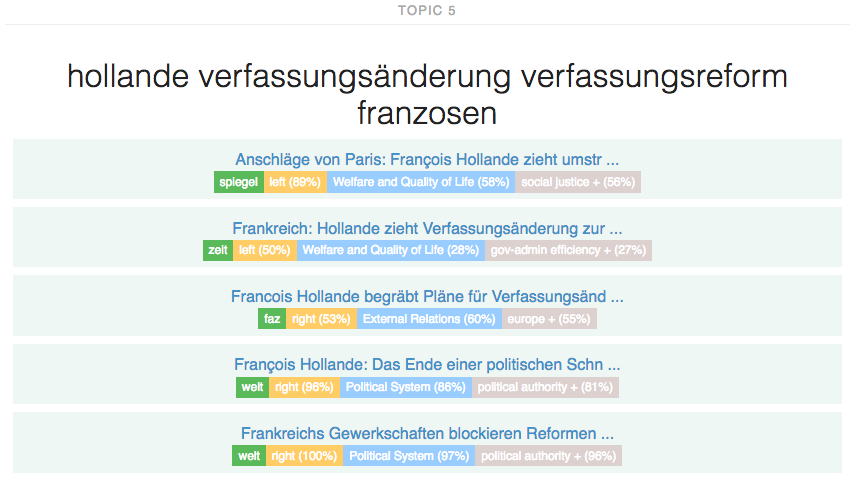
\includegraphics[width=10cm]{images/fipi-screenshot}
%%
%\end{center}
%\caption{
%\label{fig:fipi}
%A screen shot of an example web application using the political view prediction combined with topic modelling to provide a heterogeneous overview of a topic. }
%\end{figure}


\section{Conclusions and Limitations}\label{sec:conclusion}
Evaluating classifiers trained on parliament speeches we find that automated political bias prediction is possible with above chance accuracy in some cases even beyond the training text domain. These results encourage to use such systems as assistive technology for instance for human annotators in an active learning setting. 

We find a strong effect of text length and text domain on the generalization performance of the classifier, as also shown in other studies on similar data \cite{Yu2008, Hirst2014}. The first effect, longer texts are easier to classify, makes intuitive sense. Also humans are worse at judging the political bias of shorter texts out of context: Benoit et al. (2015), for example, found in an experiment where experts where differentiating whether specific sentences were dealing with economic or social policy only about 35\% agreement between all expert coders. However short texts are a realistic challenge for automated political bias prediction systems: Often political texts from social media data and other web media are indeed very short. But political education would benefit from automatic analyses of these data streams; these media have strong influence on public opinions yet are difficult to analyse with human annotators due to the large volume of data. \\
The second effect, drop in generalization performance on out-of-domain data, can be alleviated by aggregating texts into longer segments. In the case of party affiliation prediction, the out-of-domain classification is on par or even better than the prediction accuracy on in-domain data. However in the binary classification setting (government membership), aggregating manifesto data, which was written without the knowledge of which party would be member of the government, into longer texts does not counteract the effect of out-of-domain classification. We attribute this effect in part to the fact that sentiment appears to be a discriminative feature for government membership. 

\subsection*{Acknowledgements}
We would like to thank Friedrich Lindenberg for factoring out the \url{https://github.com/bundestag/plpr-scraper} from his Bundestag project. Michael Gaebler provided helpful feedback on an earlier version of the manuscript. \\
%
\newpage
\small{
\bibliographystyle{plain}
\bibliography{political_bias_prediction}
}


\end{document}
